
%(BEGIN_QUESTION)
% Copyright 2011, Tony R. Kuphaldt, released under the Creative Commons Attribution License (v 1.0)
% This means you may do almost anything with this work of mine, so long as you give me proper credit

An important pump in a chemical process is turned by an electric motor, and operators want to have visual indication in the control room that the pump is indeed turning.  There is no way to attach a speed switch to the pump shaft (that would be too easy!).  Instead, someone has installed a proximity switch near the pump shaft, situated to pick up the passing of a keyway in the shaft with each rotation.  Thus, the proximity switch will output a ``pulse'' signal when the pump shaft is spinning:

$$\includegraphics[width=15.5cm]{i03838x01.eps}$$

Operators wanted the indicator light in the control room to blink when the pump is running, for an indication of shaft motion.  The problem is, the shaft turns much too fast (approximately 1750 RPM) to directly drive the indicator with the proximity switch signal, and so an Allen-Bradley PLC was programmed to produce a slower blink using this program:

$$\includegraphics[width=15.5cm]{i03838x02.eps}$$

Explain how this program works to fulfill the function of a {\it frequency divider}, converting the high-speed pulse signal of the proximity switch into a low-speed blink for the operator light.  

\vskip 20pt \vbox{\hrule \hbox{\strut \vrule{} {\bf Suggestions for Socratic discussion} \vrule} \hrule}

\begin{itemize}
\item{} Explain how a {\it frequency divider} circuit built out of J-K flip-flop integrated circuits functions, and then describe how this PLC program is similar in principle.
\item{} Explain how to speed up the blinking rate of the light for any given motor shaft speed.
\end{itemize}

\underbar{file i03838}
%(END_QUESTION)





%(BEGIN_ANSWER)

Hint: the contact address {\tt C5:0.ACC/13} refers to the 13th bit of the counter's accumulator register, which is a 16-bit binary number.  The 15th bit would be the MSB, while the 0th bit is the LSB.

%(END_ANSWER)





%(BEGIN_NOTES)

If a pulse signal drives a binary counter, the bits of that counter's accumulator value will oscillate at sub-harmonic frequencies.  The LSB will oscillate at exactly one-half the frequency of the input; the next higher-order bit at exactly one-quarter the input frequency; the next higher-order bit at exactly one-eighth the input frequency; etc.

\vskip 10pt

By monitoring bit 13 of the counter's accumulator value, the frequency is divided by a factor of $2^{14}$, which is $1 \over 16384$.  If the shaft speed is exactly 1750 RPM (switch signal frequency = 29.1667 Hz), then the light's blinking frequency will be 0.00178 Hz, or 0.1068 times per minute.  This is very slow (9.36 minutes per on/off blink cycle!), and should probably be sped up for practical reasons.


%INDEX% PLC, ladder logic program analysis and explanation (Allen-Bradley)

%(END_NOTES)


